
\begin{frame}
  \frametitle{Testing Protocol}
  \textbf{Maximum Log Likelihood:}
  \begin{enumerate}
    \footnotesize
    \item Training database broken up into 10k segments (CHTC)
    \item Every training database entry is tested
    \item Testing sample removed from DB during each calculation
    \item Entire set of labels (reactor type, burnup, etc) predicted at once
  \end{enumerate}
  \textbf{Scikit-Learn Algorithms:}
  \begin{enumerate}
    \footnotesize
    \item Scale training data ($0$ mean and unit variance)
    \item 5-fold cross validation is used to iteratively remove 20\% of the training set as a testing set
    \item \texttt{fit} and \texttt{predict} takes place, ground truth and predictions are tracked
    \item Each label is predicted separately
  \end{enumerate}
  \textbf{SFCOMPO Testing with Nuclide Mass Training Set:}
  \begin{enumerate}
    \footnotesize
    \item After filtering out for irrelevant cases, 505 test entries remain
    \item Training set units are converted to $mg/gU_i$
    \item In scikit, scaling is applied to the training set and testing set features
    \item MLL converts the units but doesn't require scaling
    \item Time since irradiation not included in SFCOMPO
  \end{enumerate}
\end{frame}

\begin{frame}
  \frametitle{Reactor Type Classification Performance}
  \textbf{Accuracy Metrics:} \cite{scikit}
  \vspace{2mm}
  \begin{itemize}\addtolength{\itemsep}{0.4\baselineskip}
    \item $\textit{accuracy} = \frac{1}{N_\text{samples}} \sum_{i=1}^{N_\text{samples}} 
                               \mathbb{I}(y_{pred,i} = y_{true,i})$
    \item $\textit{balanced-accuracy} = \frac{1}{\sum_{i}{w_i}} \sum_{i=1}^{N_\text{samples}}
                                        w_i \cdot \mathbb{I}(y_{pred, i} = y_{true, i})$ \\
          \hspace{1.1cm} where: $w_i = \frac{1}{\sum_j{\mathbb{I}(y_j = y_i) w_j}}$
    \item Confusion matrices: 
  \end{itemize}
  \begin{figure}
    \centering
    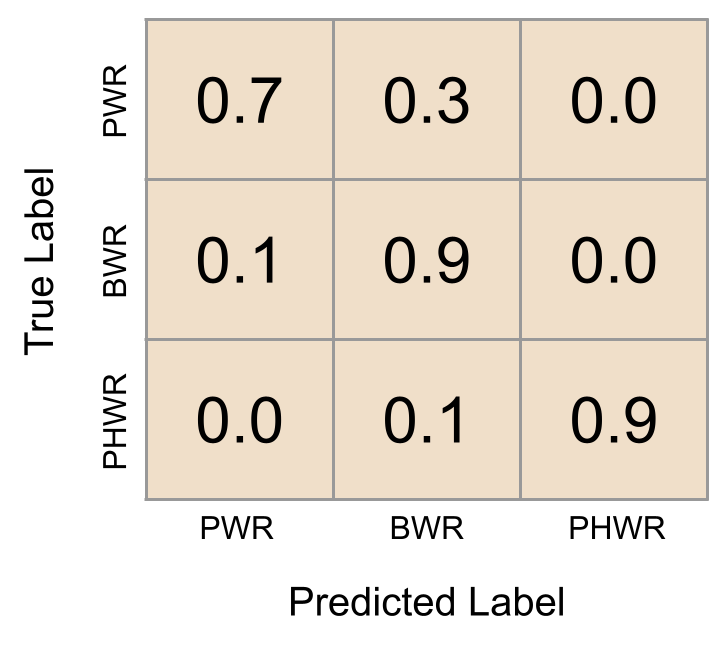
\includegraphics[width=0.34\linewidth]{./figures/cm_example.png}
    \caption{Example of a confusion matrix for the three reactor types}
  \end{figure}
\end{frame}

\begin{frame}
  \frametitle{Performance Measures for Regression}
  \textbf{Regression Metrics:} \cite{scikit}
  \vspace{2mm}
  \begin{itemize}\addtolength{\itemsep}{0.4\baselineskip}
    \item Mean Absolute Error:\\ \vspace{2mm}
          $\textit{MAE} = \frac{1}{N_{\text{samples}}} \sum_{i=1}^{N_{\text{samples}}} \left| y_{true, i} - y_{pred, i} \right|$
    \item Median Absolute Error:\\ \vspace{2mm}
          $\textit{MedAE} = \text{median}(\mid y_{true, 1} - y_{pred, 1} \mid, \ldots, 
                                          \mid y_{true, n} - y_{pred, n} \mid)$
    \item Mean Absolute Percentage Error:\\ \vspace{2mm}
          $\textit{MAPE} =  \frac{100}{N_{\text{samples}}} \cdot 
                            \sum_{i=1}^{N_{\text{samples}}}
                            \frac{\left| y_{true, i} - y_{pred, i} \right|}{y_{true, i}}$
  \end{itemize}
\end{frame}

